\documentclass{article}

\usepackage[utf8]{inputenc}
\usepackage[T1]{fontenc}
\usepackage{lipsum}
\usepackage{graphicx}
\usepackage{amsmath}
\usepackage[margin=1in]{geometry}
\usepackage{titlesec}
\usepackage{parskip}

\titleformat{\section}
{\LARGE\bfseries}{\thesection}{1em}{}

\titleformat{\subsection}
{\Large\bfseries}{\thesection}{1em}{}

\begin{document}

\pagestyle{empty}

\section*{Programmazione ad attori}
\large

\textbf{Erlang} è considerato il linguaggio che ha ridefinito la programmazione ad attori. Quando oggi si parla di programmazione ad attori, ci si riferisce essenzialmente al modello implementato da Erlang.

L'altro linguaggio di programmazione che aderisce completamente al paradigma di programmazione ad attori è \textbf{Elixir}.

Elixir ed Erlang sono sostanzialmente lo stesso linguaggio di programmazione, dove Elixir introduce una sintassi più familiare e simile ai linguaggi mainstream, oltre ad arricchire il linguaggio con costrutti aggiuntivi rispetto a Erlang. Il nucleo del linguaggio e il modello di programmazione ad attori sono identici a quelli di Erlang, poiché entrambi condividono lo stesso runtime.

La programmazione ad attori è una tecnica per sviluppare \textbf{programmi distribuiti}, ossia programmi che eseguono concorrentemente con thread che possono trovarsi su macchine distribuite in una rete. Per implementare sistemi distribuiti, la programmazione ad attori rimane il paradigma più efficace mai sviluppato.

Esistono anche numerose librerie che permettono di utilizzare la programmazione ad attori in linguaggi mainstream, come ad esempio librerie per Java e Scala (la libreria \textit{Akka}).

Questo approccio ibrido, tuttavia, non è sempre consigliabile. Quando si tenta di integrare costrutti da due paradigmi diversi in un unico linguaggio di programmazione, l'idea intuitiva è che si ottenga una soluzione migliore rispetto ai due paradigmi originali, poiché si possono sfruttare entrambi. In realtà, combinare costrutti da paradigmi diversi è generalmente problematico.

Ciò accade perché quando si scrive un frammento di codice, si garantiscono determinate proprietà dell'output basandosi sulle garanzie delle proprietà dell'input. Un linguaggio multiparadigma che permette di combinare diversi costrutti può sembrare semplificare la produzione di output con certe garanzie. Il problema è che questo indebolisce le garanzie in input.
Per esempio, in un linguaggio funzionale puro, dove non esiste mutabilità delle strutture dati, si ha la garanzia che il dato non possa essere modificato da altri. Questa garanzia è fondamentale perché sapere che certe parti del dato rimangono immutate è la chiave che consente di ottenere algoritmi con una determinata complessità computazionale asintotica nei linguaggi funzionali. Introdurre costrutti imperativi che possono modificare i dati comporta la perdita di questa garanzia.

Un linguaggio di programmazione, o un paradigma, è caratterizzato sia da ciò che permette di fare, sia soprattutto da ciò che \textit{non permette di fare}, ovvero dalle salvaguardie che mette a disposizione.

Combinare paradigmi indebolisce queste garanzie e quindi non sempre rappresenta la soluzione ottimale.

Erlang è un linguaggio di programmazione \textbf{funzionale}. All'interno della famiglia dei linguaggi di programmazione funzionali, Erlang si distingue per essere \textbf{non tipato}, caratteristica estremamente rara, considerando che la maggior parte dei linguaggi funzionali moderni è tipata.

Inoltre, Erlang è relativamente più vicino al basso livello rispetto ad altri linguaggi simili. Si può considerare Erlang come l'\textbf{assembly} dei linguaggi di programmazione funzionali.

Erlang non nacque originariamente come linguaggio di programmazione ad attori, ma riscoprì questo paradigma successivamente alla sua creazione nel 1976. Oggi, quando si parla di programmazione ad attori, si fa riferimento essenzialmente a Erlang.

Al centro della programmazione ad attori vi è il concetto stesso di \textbf{attore}. Un attore è caratterizzato da tre componenti principali:
\begin{itemize}
    \item \textbf{PID (Process Identifier)}: identificatore univoco dell'attore. È un \textit{nome logico} che indica come raggiungere l'attore. L'unico modo per comunicare con un attore, la cui posizione è nascosta dal linguaggio, è conoscere il suo nome logico. Solo chi conosce il nome logico di un attore può comunicare con esso.
    \item \textbf{Mailbox}: coda per la ricezione dei messaggi. Un attore riceve messaggi e li inserisce in questa coda.
    \item \textbf{Behaviour}: funzione che elabora i messaggi trasformandoli in una lista di azioni e in un nuovo behavior. Ogni volta che viene ricevuto un messaggio, il behavior può cambiare completamente. Essendo una funzione, ad ogni messaggio ricevuto corrisponde una lista di azioni e un nuovo comportamento da adottare. Le azioni possono includere anche computazioni interne.
\end{itemize}
L'attore può inviare messaggi in maniera asincrona ad altri attori di cui conosce il PID. L'invio è esclusivamente \textbf{asincrono}, quindi non esiste sincronizzazione. Quando si invia un messaggio, non si sa se o quando verrà ricevuto. Questa è l'unica forma di comunicazione in Erlang. Inoltre, un attore può creare altri attori.

Un attore corrisponde a un \textbf{singolo thread di computazione}, quindi all'interno di un attore non possono esistere thread multipli.

La programmazione ad attori è un caso particolare di programmazione \textbf{reattiva} o \textbf{event-driven}. Immaginiamo un sistema composto da decine di migliaia, centinaia di migliaia, o persino milioni di attori. WhatsApp, ad esempio, fu inizialmente implementato in Erlang. Ogni singola applicazione WhatsApp installata corrisponde a un attore, quindi il sistema comprendeva milioni di attori. Il numero di attori in un sistema tende generalmente ad aumentare nel tempo.

Non bisogna tuttavia pensare che tutti gli attori siano costantemente impegnati in calcoli. Quando un attore riceve un messaggio, esegue brevemente una serie di operazioni, eventualmente generando altri messaggi, per poi tornare in stato di attesa. La programmazione ad attori è quindi ideale per configurazioni con un numero elevatissimo di attori, di cui solo una piccola parte è attiva contemporaneamente. Questo rappresenta l'approccio opposto alla programmazione multithreading tradizionale, dove il numero di thread deve essere contenuto poiché ogni thread è costoso e l'avvio di troppi thread rallenta significativamente il sistema.

Gli attori non condividono risorse: né stato né memoria, anche quando sono eseguiti sulla stessa macchina e collaborano tramite scambio di messaggi.

Un \textbf{sistema di attori} è un sistema complesso composto da molteplici attori in esecuzione. L'esecuzione è indipendente dalla posizione fisica degli attori e la topologia della rete può variare. Gli attori possono essere eseguiti in modo completamente trasparente sullo stesso nodo, sulla stessa macchina virtuale, sullo stesso core o sulla stessa CPU. Questo significa che in Erlang non esiste una reale distinzione tra programmazione concorrente su una singola macchina, programmazione distribuita o programmazione parallela.

Uno dei principali punti di forza della programmazione ad attori di Erlang è aver fornito una soluzione radicale ma estremamente efficace alla gestione dei guasti.

\subsection*{Esempio pratico in Erlang}
Erlang condivide elementi della sua sintassi con il linguaggio di programmazione logica Prolog. Ecco un esempio di attore per la gestione di un conto corrente:
\begin{center}
    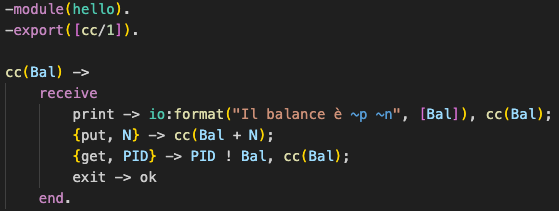
\includegraphics[width=1\textwidth]{img/hello_code.png}
\end{center}
Il primo passo è la dichiarazione del \textbf{module}, il cui nome deve corrispondere al nome del file. In Erlang, una riga che inizia con il simbolo \textbf{-} rappresenta una direttiva, che non fa parte del codice eseguibile ma fornisce istruzioni al compilatore.

Un secondo aspetto importante è che all'interno di un modulo Erlang vengono definite funzioni, che possono essere esportate o meno tramite la direttiva \textbf{export}. Questo meccanismo permette di scegliere quali funzioni rendere accessibili dall'esterno e quali mantenere interne al modulo. Tutto ciò che non viene esportato rimane nascosto. 

La direttiva export accetta una lista di funzioni da esportare, dove ogni funzione è indicata dal suo nome seguito dal numero di parametri che richiede. Questo è necessario perché possono esistere funzioni con lo stesso nome ma differenziate dal numero di parametri.

In Erlang, tutte le istruzioni, i comandi e le definizioni terminano con un \textbf{punto}.

Quando si definisce un attore, occorre definire il suo behavior. Il behavior deve specificare cosa fare quando si ricevono determinati messaggi.

Il nostro conto corrente deve avere un \textit{balance}, che indica il saldo disponibile. Dopo aver ricevuto un messaggio, l'attore deve acquisire un nuovo behavior.

In Erlang, il behavior viene definito da una funzione, tipicamente ricorsiva. Questa funzione ricorsiva prende in input lo stato attuale (in questo caso, il saldo corrente), descrive come reagire ai messaggi e, dopo averne ricevuto uno, adotta un altro behavior. Nel nostro esempio, il behavior rimane lo stesso: vogliamo che il conto corrente continui a ricevere messaggi.

Erlang non permette mutazioni, tranne in alcuni costrutti specifici. Le variabili, una volta definite, non possono essere modificate, comportandosi essenzialmente come costanti.

Un behavior viene descritto all'interno di un costrutto \textbf{receive-end}.

Il behavior deve specificare: se ricevo un certo messaggio, eseguo una certa azione. Questo viene implementato tramite una serie di pattern che vengono confrontati con i messaggi nella mailbox in un determinato ordine. Se nella mailbox viene trovato un messaggio che corrisponde a un pattern, viene eseguito il codice associato.

Un pattern è una descrizione, una possibile forma dell'input. Ogni pattern può corrispondere o meno a un messaggio nella mailbox che ha la stessa forma. Inoltre, quando un pattern corrisponde a un messaggio nella mailbox, le variabili nel pattern vengono associate ai valori corrispondenti nel messaggio.

Come sono strutturati questi pattern? 

I pattern \textit{print} ed \textit{exit} corrispondono semplicemente alla ricezione di messaggi contenenti i rispettivi atomi.

Anche questi sono scritti con lettere minuscole, come \textit{cc}, ma senza parentesi tonde.

Con la lettera minuscola e parentesi tonde si indica una funzione. Senza parentesi, si tratta di un \textbf{atomo}.

Un atomo è un tipo di dato che ha come unica proprietà quella di essere uguale a se stesso e diverso da tutti gli altri atomi. Gli atomi vengono utilizzati per distinguere diversi tipi di messaggi.

Passiamo al pattern \textit{put}, dove il messaggio deve contenere anche l'importo da versare. In questo caso, il messaggio è una coppia di valori dove il primo elemento è l'atomo put e il secondo è una variabile (indicata con lettera maiuscola). Questo consente di effettuare il \textbf{pattern matching}.

Si noti come non viene modificato direttamente il valore del saldo: non c'è una modifica imperativa del balance, ma una chiamata ricorsiva con un nuovo valore.

All'interno del caso \textit{print}, si può osservare la separazione tra istruzioni.

In Erlang, le istruzioni sono separate da \textbf{virgole}, mentre i diversi casi di pattern matching sono separati da \textbf{punto e virgola}.

Per quanto riguarda \textit{exit}, l'obiettivo è terminare l'esecuzione dell'attore. Viene quindi restituito un valore di uscita, che può essere qualsiasi cosa.

Per il caso \textit{get}, per ottenere informazioni sul proprio conto corrente, è necessario conoscere il PID del richiedente. In questo modo, l'attore saprà a quale PID inviare il risultato della richiesta. La sintassi successiva permette di inviare al PID richiedente il valore del saldo.

Passiamo ora all'esecuzione del codice.

Erlang è simile a Java: il codice viene compilato e poi eseguito da una macchina virtuale (chiamata \textbf{Beam}). Generalmente, su ogni macchina fisica è in esecuzione una singola macchina virtuale, chiamata \textbf{nodo}, anche se nulla impedisce di avere più macchine virtuali su una stessa macchina fisica.

Quando si avvia il nodo della macchina virtuale, viene anche avviata una \textbf{shell}, che permette di impartire comandi e visualizzare risposte. Anche la shell è un attore.

Ogni volta che si avvia un attore, è possibile interagire con esso tramite la shell. Ad esempio, dalla shell si può avviare l'attore del conto bancario e poi comunicare con esso.

Il principio fondamentale è che in Erlang tutto è un attore.

Come detto in precedenza, il primo passo è compilare il codice. È disponibile una funzione chiamata \texttt{c(nome\_file)}, che consente di compilare il file specificato. La compilazione ha successo se non vengono rilevati errori.

Una volta compilato, il modulo viene caricato automaticamente dalla macchina virtuale e le sue funzioni diventano disponibili.

Per creare un attore con quel behavior, si può utilizzare il comando \texttt{spawn(nome\_modulo, nome\_funzione, lista\_argomenti)} (NB: la funzione spawn ha diverse varianti sintattiche; qui ne utilizziamo solo una).

Questo comando restituisce il PID dell'attore appena creato. Questo PID non è necessariamente lo stesso su tutti i nodi, ma il runtime riesce sempre a indirizzare correttamente l'attore corrispondente.

Per interagire con l'attore, è sufficiente eseguire dalla shell comandi come \texttt{PID ! print.}, che restituirà il saldo del conto.

Analogamente, \texttt{PID ! \{put, 2\}.} aggiornerà il saldo del conto corrente.

Per la \texttt{get}, la situazione è leggermente diversa. Apparentemente, non si riceve una risposta immediata alla richiesta effettuata. Questo accade perché la shell è un attore particolare. La shell è un attore che differisce dagli altri, perché mentre gli attori normali hanno un behavior che risponde ai messaggi ricevuti, la shell ha una sorta di secondo behavior che elabora ciò che viene digitato sullo standard input anziché i messaggi nella sua mailbox. Il messaggio ricevuto viene inserito nella mailbox della shell, ma non viene elaborato automaticamente.

Per estrarre il messaggio dalla mailbox, occorre fornire un behavior temporaneo alla shell, ad esempio con il comando \texttt{receive MSG -> MSG end.}

Questo approccio di programmazione riflette la logica originale della programmazione ad attori del 1976, prima delle varie estensioni introdotte da Erlang.

\subsection*{Erlang}
Il linguaggio Erlang è progettato attorno al concetto di programmi concorrenti che vengono eseguiti per periodi estremamente lunghi, con concorrenza massiva (>= 100.000 attori).

Permette anche di sviluppare sistemi distribuiti, con la possibilità di aggiornare il codice durante l'esecuzione senza interrompere il programma.

Incorpora inoltre sofisticati meccanismi per la gestione dei guasti, che rendono Erlang ideale per applicazioni che richiedono runtime "infiniti" (come gli switch Ericsson con software scritto in Erlang, che raggiungono un uptime del 99,999999\%).\vspace{14pt}\\

Le principali scelte progettuali di Erlang sono:
\begin{itemize}
    \item \textbf{Nessuna memoria condivisa}, lock o mutex, poiché ciò comporterebbe una gestione eccessivamente complessa e non funzionerebbe efficacemente in scenari distribuiti. Inoltre, il meccanismo della memoria condivisa è problematico dal punto di vista della tolleranza ai guasti, dato che un thread che fallisce dopo aver acquisito un lock potrebbe causare deadlock.
    \item \textbf{Scambio di messaggi asincrono}, con ricezione potenzialmente non sequenziale. L'ordine di ricezione dei messaggi in uno scenario distribuito non è garantito. Se un messaggio viene estratto dalla mailbox in un momento non opportuno, deve essere elaborato esplicitamente in un secondo momento.
    \item \textbf{Tolleranza ai guasti tramite "Let it fail!"}. La gestione degli errori è particolarmente complessa in scenari distribuiti, a causa di potenziali deadlock causati da messaggi persi o processi remoti irraggiungibili. Il principio "Let it fail" stabilisce che, in presenza di errori, un processo e tutti quelli strettamente connessi ad esso vengano terminati. Dopo la terminazione, un supervisore si occupa di riavviare i processi interrotti.\\
    L'idea è quella di strutturare la computazione in modo gerarchico. Invece di risolvere direttamente un problema, un attore genera una serie di attori figli. Questi attori figli collaborano tra loro per risolvere il problema.\\
    L'attore padre si pone in uno stato di supervisione, osservando i figli e attendendo la loro terminazione. Se uno dei figli fallisce per qualsiasi motivo, questo comporta la terminazione di tutti i suoi fratelli e di eventuali discendenti. Il padre, osservando la terminazione dei figli, può riavviare la computazione. Naturalmente, se dopo ripetuti tentativi di riavvio la situazione non migliora, il padre stesso terminerà, causando a sua volta la terminazione di tutti i suoi fratelli e così via fino all'attore radice.\\
    Questo approccio funziona particolarmente bene se il padre è in grado di ricreare i figli con lo stato che avevano al momento del fallimento. Nei linguaggi funzionali privi di mutazione come Erlang, quando il padre crea i figli, il suo stato non viene alterato dai figli stessi, poiché la memoria non viene mai modificata ma si crea sempre nuova memoria.\\
    Quindi, quando i figli vengono terminati, il padre può ricrearli in tempo O(1), senza dover ricorrere a tecniche di backtracking o ricreazione dello stato: il padre possiede esattamente lo stato in cui si trovava quando ha creato i figli la prima volta e può quindi ricrearli rapidamente.
\end{itemize}
La macchina virtuale di Erlang, chiamata \textbf{Beam}, viene eseguita come unico processo kernel multi-threaded, con un thread per core.

Per ogni attore è presente un \textbf{Language Thread}. Il sistema operativo non ha consapevolezza degli attori, che vengono schedulati sui kernel thread con un bilanciamento del carico automatico.

Il cambio di contesto (Context Switch) per i language thread è estremamente leggero. Erlang implementa un cambio di contesto collaborativo, dove la macchina virtuale si occupa di gestire i vari cambi di contesto. Si parla in questo caso di \textbf{green thread}, che utilizzano risorse minime.

Anche l'impronta di memoria (Memory Footprint) dei language thread è estremamente contenuta: un nuovo attore nasce occupando circa 300 parole di memoria. Questo permette di gestire centinaia di migliaia di attori contemporaneamente. Gli attori Erlang iniziano con un utilizzo minimo di memoria, senza uno stack preallocato.

Lo stack cresce dinamicamente quando necessario, creando uno stack di dimensione 2N e copiandovi il contenuto dello stack precedente. Questo ha un costo computazionale ammortizzato \textbf{lineare O(n)}.

Questo costo riguarda solo il momento della creazione del nuovo stack; negli altri casi, il costo ammortizzato è \textit{O(1)}. Ciò consente di gestire milioni di language thread simultaneamente.

Un'altra caratteristica fondamentale è l'\textbf{hot code swap}, ovvero la possibilità di caricare a runtime una nuova versione del codice senza interrompere l'esecuzione del programma.

La libreria standard di Erlang è denominata \textbf{OTP (Open Telecom Platform)}, che include tutto il necessario per implementare software distribuiti, come componenti client-server generici.

Al suo interno è presente anche un database distribuito chiamato \textbf{Mnesia}, che permette ad ogni attore di ogni nodo di leggere e scrivere sul database distribuito come se stesse operando sulla memoria locale. Il vantaggio di questo approccio risiede nel fatto che le diverse istanze di Beam comunicano continuamente tra loro, propagando le informazioni. Questo garantisce un alto livello di coerenza dei dati. Naturalmente, questo sistema non è immune da possibili guasti o fallimenti: non è garantito che ciò che viene scritto in un nodo sia immediatamente visibile in un altro nodo.

\subsection*{Elixir}
Elixir è un linguaggio ad attori implementato sulla stessa macchina virtuale Beam di Erlang. La sua sintassi si ispira a Ruby, mentre quella di Erlang deriva da Prolog.

Elixir arricchisce Erlang con:
\begin{itemize}
    \item \textbf{Metaprogrammazione}: consente a un programma di controllare e manipolare il proprio codice. In altre parole, permette di scrivere programmi che generano o modificano altri programmi (o se stessi) durante la compilazione o l'esecuzione.
    \item \textbf{Macro igieniche}: garantiscono che le variabili introdotte nella macro non interferiscano con quelle già esistenti nel codice in cui vengono espanse. Il compilatore o l'interprete assicura l'unicità delle variabili, evitando problemi di scope e collisioni di nomi.
    \item \textbf{Polimorfismo tramite protocolli}: un sistema flessibile per implementare comportamenti polimorfici senza ereditarietà.
\end{itemize}
\end{document}